\chapter{Preliminary Evaluation}
To evaluate the above mentioned research questions, a small pilot study was conducted. Optimising and improving our approach with the help of feedback from a small team consisting of knowledge workers is the main goal of this master thesis. Further, by collecting additional data hope to get valuable first insights into the following areas:

\begin{enumerate}
    \item Common workflows and patterns \\
          \textit{RQ1:} How do knowledge workers use and interact with AmbientTeams? How do they integrate it into existing workflows?
    \item Mood sharing behavior \\
          \textit{RQ2:} Do knowledge workers want to share their moods with their remote team members? If so, what causes knowledge workers to share their moods with their team?
    \item Feeling of isolation \\
          \textit{RQ3:} Can a people-focused team mood and status sharing approach decrease the feeling of isolation in remote knowledge worker teams?
    \item Information consumption \\
          \textit{RQ4:} What do knowledge workers learn from information shared by their team members? What kind of information is the most valuable?
\end{enumerate}

The data used to answer the above research questions came from three different sources. Given the relatively few participants, it was important to have both quantitative and qualitative data. After having a look at the study procedure in the next chapter, each of the three data sources and their relevance for the research questions are elaborated.

To find participants, a recruitement flyer (see .) The study was conducted with two knowledge worker teams, each team fulfilling the following paritication requirements:

\begin{enumerate}
    \item At least three team members
    \item Three or more common working days a week
    \item Spending the majority of their work day on the computer
    \item Having all the required rights to install AmbientTeams on their work computer
    \item Willingness to use AmbientTeams during at least 3 full days of work (approximately 0800 - 1700)
    \item Using macOS or Microsoft Windows
    \item An active internet connection
\end{enumerate}

\section{Procedure}

\begin{figure}[h]
    \centering
    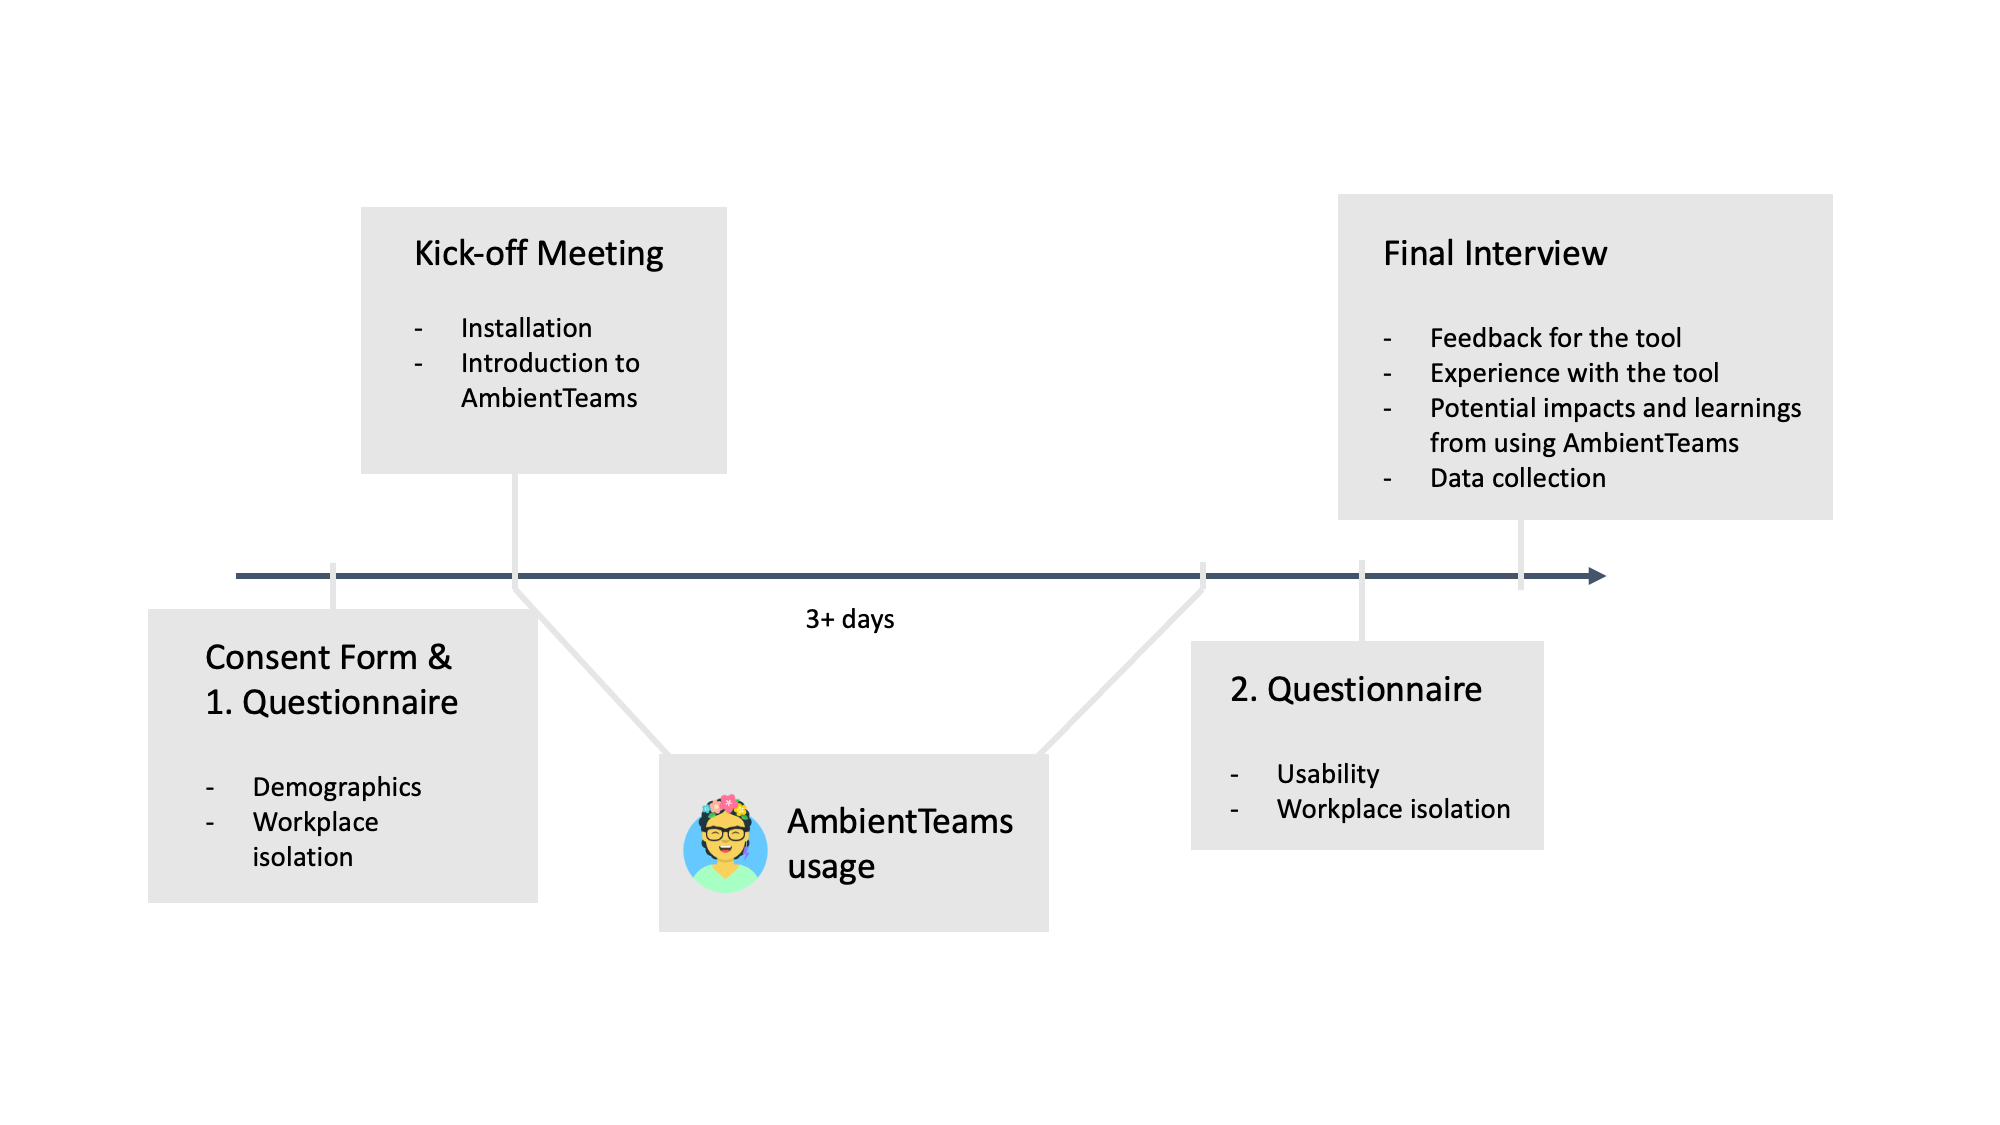
\includegraphics[width=.8\linewidth]{./images/Study_Timeline.png}
    \caption{Study timeline}
    \label{fig:study_timeline}
\end{figure}

\begin{enumerate}
    \item Initial meeting: Installation, registration, team creation, give each team member a participant ID (see \autoref{section:initial_meeting})
    \item Pre-study questionnaire (see \autoref{section:questionnaires})
    \item Evaluation phase (see \autoref{section:evaluation})
    \item Post-study interview (see \autoref{section:interview}) with data collection (see \autoref{section:data_collection})
    \item  Post-study questionnaire (see \autoref{section:questionnaires})
\end{enumerate}

\section{Initial meeting}
\label{section:initial_meeting}
Installation

\section{Pre- and post-study Questionnaires}
\label{section:questionnaires}
The pre and post study questionnaires are used to asses the feeling of workplace isolation before and after the evaluation period. The questions are taken from ....

\section{Evaluation Phase}
\label{section:evaluation}
How long? \\
During the study notes from notion

\section{Interview}
\label{section:interview}
Interview questions and their relevance for the research questions

\section{Data Collection}
\label{section:data_collection}
\autoref{table:data_collection} shows an overview of all data collected and for which research question they are relevant.

\begin{table}[h]
    \centering
    \begin{tabular}{ |c|c|c| }
        \hline
        Data collected & Storage & Relevant for \\
        \hline
        cell4          & Local   & cell5        \\
        cell7          & Local   & cell8        \\
        \hline
    \end{tabular}
    \caption{The data collected during the preliminary evluation and its relevance for the RQs}
    \label{table:data_collection}
\end{table}